\section{Android app architecture}
\todo{Fix refs}
The app runs on the user`s Android device and was designed to run on Android version 4.0 or greater. As of March 2014 this makes up for 79,7\% of all Android devices~\cite{AndroidDeviceFragmentation}.
The team decided to only adapt the app for these version's because the app is a proof-of-concept, and the team assumed that the relevant user's would have a relatively modern phone. Making the app more backward compatible would demand more work and extra support libraries. 

\subsection{Best practice}

The best practice guidelines for Android~\cite{androidPracticePerformance} states that one should avoid using a complex architecture. A complex architecture would require a larger code base, and the complexity is often not needed in an app. However, design decisions still need to be made. 
By having concise code guidelines, and reasonable use of tools would keep the development process as simple, effective, and bug free as possible. 

The functionality of the app would demand a lot data storage and transactions. Data is stored in an internal SQLite database. Data transactions takes time and blocks the thread it's running on.
Android does UI rendering on the main thread. Thus, by running long operations on the main thread, the entire app interface will be unresponsive. That must be avoided at all cost to not destroy the user experience. The app also needs to handle user authentication and data backup on the remote server.

The choice of how to do the architecture will thus give a large impact on the overall impression of the app. The next sections will explain how the different parts of the app work together as a process, how data is accessed and used, what patterns are used, how a user is authenticated, and data backup.

%To avoid the issue of blocking the main thread it was decided to make use of Androids built in logic for async data access, and a design pattern for business logic.

\subsection{Class structure}

An Activity is the main 'thing' in Android. It's a process with the full life-cycle of the device and the possibility to show a view to the user.

To access the different parts of the app it was decided to use a navigation drawer that is accessed through the app icon on the action bar, or with a swipe from the left. The different parts of the app is shown when the user clicks on it in the navigation drawer. Each part accessed through the navigation drawer is henceforth called a tab. The structure of how the main activity communicates with the navigation drawer is shown in figure~\ref{fig:class_diagram_drawer}.

Changing tab does not change the process. Each tab and the navigation drawer is implemented as a Fragment. A Fragment is a representation of some behavior or a interface part of the Activity. Fragments can be taken in and out of a Activity interface, or contain multiple. A sub part of the Activity life-cycle is implemented in the Fragment so it can work as a self contained module. 

\begin{figure}[H]
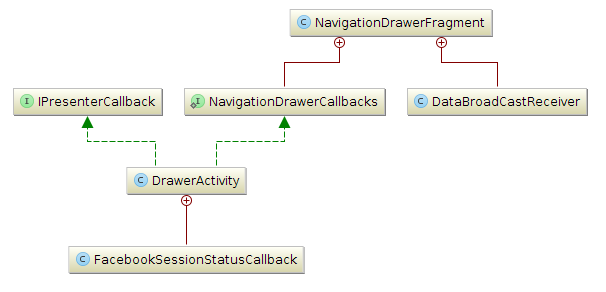
\includegraphics[width=\textwidth]{ch/architecture/fig/class_diagram_drawer.png}
\caption{Class diagram for the main Activity.}
\label{fig:class_diagram_drawer}
\end{figure}

When a tab in the navigation drawer is chosen it will use a callback to the 'DrawerActivity` class which swaps in the new Fragment to the view and closes the navigation drawer.

Each tab has it's own logic and has a default behavior defined by 'DefaultTabFragment`. A class diagram illustrating the main Fragments are shown in figure~\ref{fig:class_diagram_fragments}. The default behavior takes care of updating the name of the current tab to the Action Bar.

\begin{figure}[H]
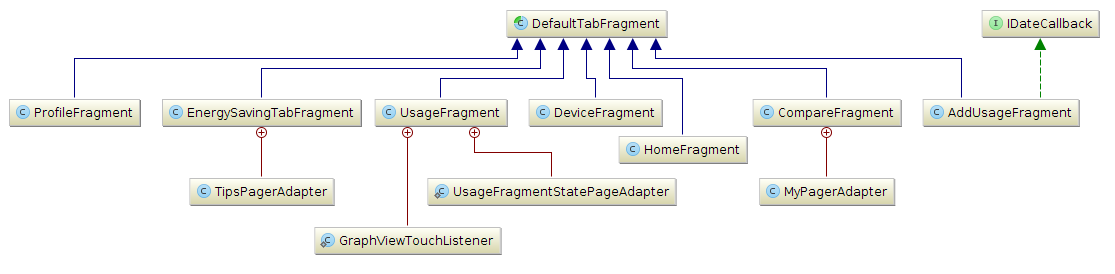
\includegraphics[width=\textwidth]{ch/architecture/fig/class_diagram_fragments.png}
\caption{Class diagram for the fragments.}
\label{fig:class_diagram_fragments}
\end{figure}

\subsection{Data access}
Data access to the underlying database is done using ContentProviders~\cite{contentproviders}. This gives the app a uniform \gls{CRUD} (abbreviation for create, read, update, and delete) access model. The data will be accessed with \gls{URI}'s (abbreviation for uniform resource identifier) that is uniquely defined. Fetching the data is done by implementing a LoaderManager~\cite{loadermanager}. LoaderManager is an interface defining callbacks to get the URI to query, how to handle data reset, and the data returned from the query. The LoaderManager runs on another thread, and thus avoids the problem of blocking the main thread from rendering the UI. It will also handle the life cycle of the data. When data related to the URI changes, the LoaderManager will load the data again. 

ContentProviders contains a lot of boilerplate code and is time consuming to code. But the upsides far outweigh the downsides. When ContentProviders are used with LoaderManager one gets a view that is automatically updated when the data changes without bothering the UI thread. Other solutions are to work directly on the SQLite driver with SQL, or use a pattern to make it work fluently. One such pattern is discussed in the next section. 

\subsection{Business logic}
After having a uniform access model to the database, the issue of where to place the actual business logic (data manipulation) must be tackled. Keeping the business logic in one generic place makes doing changes easier, and avoids the issue of knowing where every data operation is done that must be updated. Doing that can also create hard to find bugs. Following a smart design pattern will handle your business logic and make it easy to update the view. 
The team decided to use the pattern Model-View-Presenter (MVP). MVP is a Model-View-Controller (MVC) derivative~\cite{mvc}. All business logic is handled in presenter classes, between the views and models. Through this uniform access, all logic applied to data preservation (server synchronization), and data control can be handled in one place. The life cycle of the presenter classes is in the base Activity class, and all other sub fragments can get access to it though a interface. 
This pushes almost all logic into the presenters, making the code in the fragments as minimal as possible. 
MVP also makes updating the view easy when the data changes. But since all data is accessed through a ContentProvider it was possible to avoid setting up listeners. But having the possibility to do so is a good idea for further iterations of the app. But for the moment no view updating code is needed. The Presenters only handle how to manipulate the models and applies it back to the database.

\begin{figure}[H]
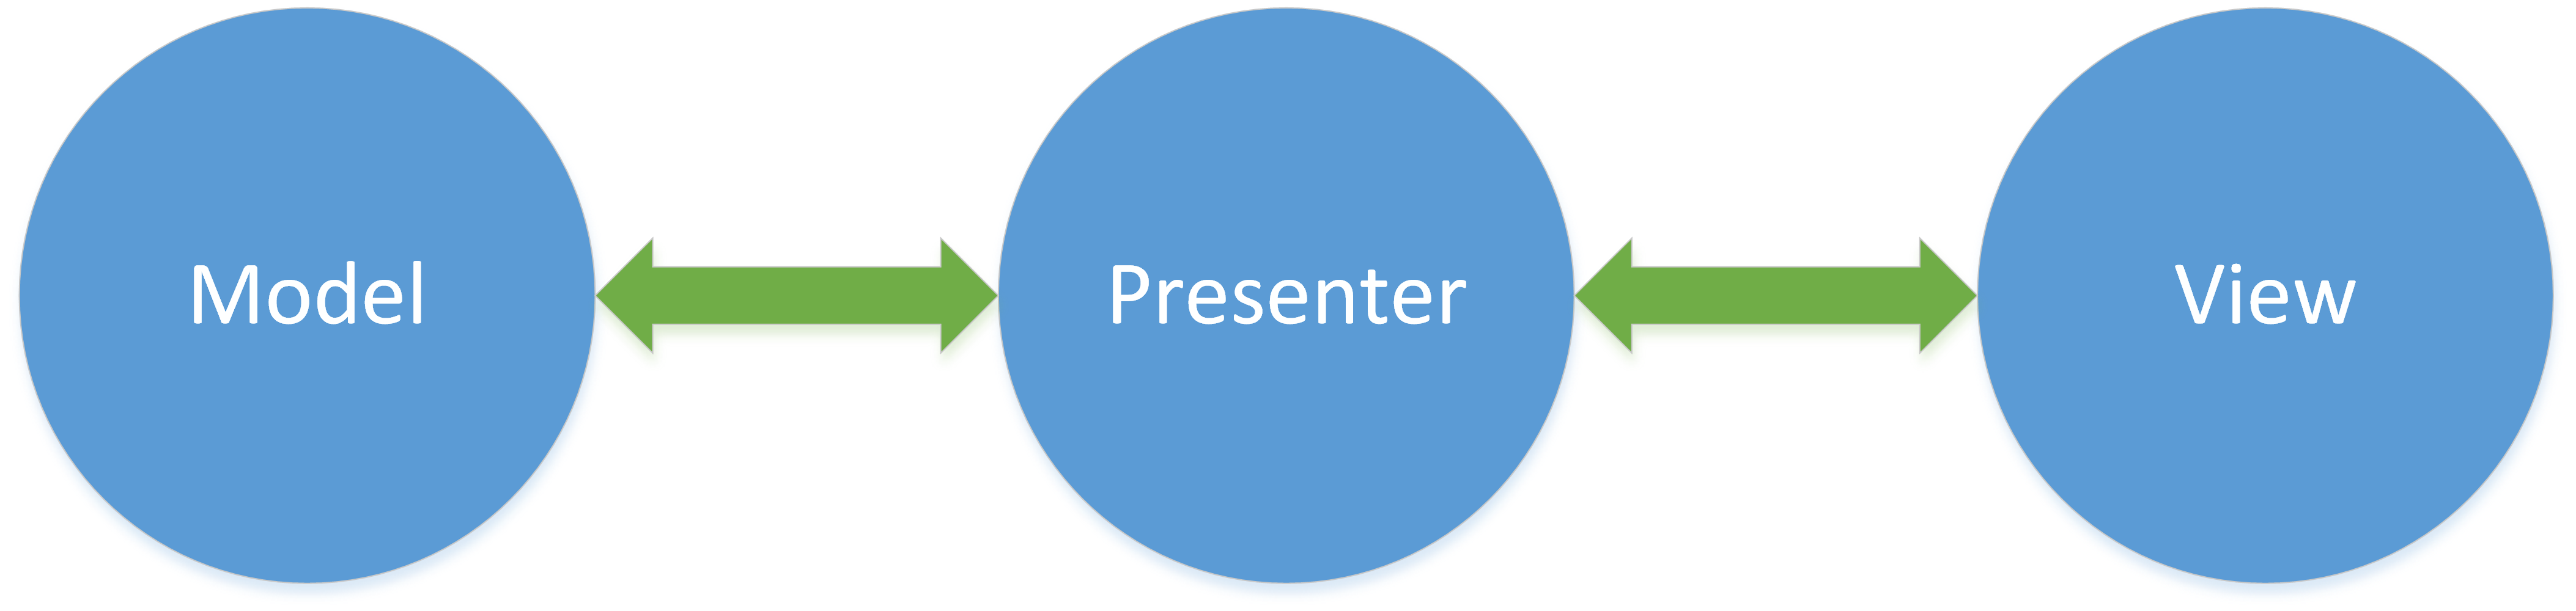
\includegraphics[width=\textwidth]{ch/architecture/fig/mvp.png}
\caption{MVP}
\label{fig:mvp}
\end{figure}

\subsection{User authentication}
The app needs to backup data on a server. Our server, as explained in chapter~\ref{sec:arch_server}, exposes a restful API were data can be backed up.

The first problem that arises with backing up data is that the user must be identified as a specific user. The choice was made not to make our own authenticator. By using a third party authenticator to handle user and user id with OAuthV2.0 we made the device authentication token based. 
For the time being the third party authenticator is Facebook and the Facebook session is maintained with the FacebookSDK for Android. 
%For the moment this is not entirely true to how it is done now. Some shortcuts were done to have a working system. But the main authentication architecture is made.
Now the a user can log in with his Facebook user and fetch data from his Facebook account, but not communicate with our server. 

The next case is how to handle the session data from Facebook. The Android system has it's own account architecture. Working with this architecture requires the app to register a AbstractAccountAuthenticator~\cite{androidAccount} class in the AndroidManifest. The AbstractAccountAuthenticator is generic and can be made to create accounts for all types of services. The token and other related data (Facebook id) returned from Facebook is stored in the account and can accessed when necessary.

Other OAuthV2.0 authentication providers can also be used (Twitter, Google, your own private OAuthV2.0 authenticator, etc). 

%For the time being only the Facebook user id is used to authenticate the user to our server.

\subsection{Server data access}

All the user data is saved on the server. Communication to server is done with a framework named Volley. It is created by Google and the source code resides within AOSP (Android Open Source Project). It is made to make communication with restful endpoints easier.

Most of all server access is done when synchronizing data with the server. 
Data synchronization is done by using Androids built in SyncAdapter. The SyncAdapter is a self-contained process that that fetches and delivers all new data to and from the server. The SyncAdapter is registered to a specific account on the Android system. The account will then provide the session data that will identify the user to the server. How the session data was acquired was explained in the last section. For the time being only the Facebook id is used when communicating with the server. This is not secure in any way. But changing this to use the token and make the server find the user id based on the token is a easy next step to make.

Communication to the database is still done through a ContentProvider. Since the changes will affect the URI, the view will get the new data and be rendered again automatically if the the app is running. 

The algorithm for how the data synchronization is done is showed as pseudo code in code snippet~\ref{fig:algorithm_sync}.

%Pseudo code for the sync

\noindent\begin{minipage}{\textwidth}
\begin{lstlisting}[caption={Algorithm for the synchronization flow.}, label={fig:algorithm_sync}]
var lastSync = Last synchronization time stamp from account
var now = Current time in Unix epoch

var localDataModels = Get all local changes after lastSync

var serverDataModels = Get all server changes after lastSync

sendLocalModelsToServer(localDataModels)

saveModelsToLocalDB(serverDataModels)

if no errors
  accountLastSync = now
\end{lstlisting}
\end{minipage}

The algorithm is straightforward and will retry data synchronization until it does not fail. The reason for that is that the synchronization time stamp only will be updated when everything goes well. If the error checking fails and the last synchronization time stamp fails, then data will be lost. 
This is not a perfect approach to synchronization, but acceptable within the time frame that it was needed. 

SyncAdapters can be configured to run when it is best suited. This is when processor is not busy and the device has WiFi Internet connection. It can also be forced to run on regular intervals.

\subsection{Keeping the code clean}

Other long running operations, for example the rendering of the graph, is a time consuming task. To avoid the main thread to be blocked in those cases AsyncTask is used. AsyncTask defines an interface to give references to objects, an operation to run on another thread, and code to run after the long operation is finished that can update the UI. 

Thereafter code written must generally continue to avoid doing wrong operations on the main thread. Forgetting to do this properly is easy. So, to enforce this, Android has a tool named StrictMode~\cite{androidStrictMode}. It can be tweaked to monitor the UI thread and check for file operations, network access and other problems. The penalty for breaking these defined rules can be set to emit a stack trace or kill the app. By having StrictMode configured while coding made discovering bad design easier. 

%The app will follow standard Android design guidelines regarding the user interface design.
